%----------------------------------------------------------------------------
\chapter{Getting started}\label{guide:start}
%----------------------------------------------------------------------------
Start these steps in your first week, alongside the research. Each step names its owner. By the first consultation, complete your account checklist and verify access to the project repository and Overleaf with both advisors as described below. Bring a problem paragraph and initial sources to that consultation. Finish the VM and bibliography integration alongside early research; optional editor and operating-system tooling must not delay the work.

%----------------------------------------------------------------------------
\section{Share your identifiers}\label{guide:start:ids}
\emph{You.} Send both of us your Neptun code, GitHub username and \texttt{@edu.bme.hu} email address by Teams or e-mail. Our faculty addresses are on the \href{https://ftsrg.mit.bme.hu/en/about/}{research group's page}. We need these identifiers to add you to Overleaf, GitHub and the Zotero group.

%----------------------------------------------------------------------------
\section{Create your ORCID iD}\label{guide:start:orcid}
\emph{You.} Create a free \href{https://orcid.org/register}{ORCID iD} in your first week, or use your existing one. ORCID gives you a persistent researcher identifier that distinguishes you from people with similar names and stays with you when you change institutions. You can register before you have any publications; see ORCID's \href{https://info.orcid.org/researcher-faq/}{researcher FAQ}.

Register with the name you intend to use on your papers. Add a personal email address that you will retain after graduation as well as your university address, and verify the addresses using ORCID's emails. Choose the visibility settings for your record; ORCID's \href{https://support.orcid.org/hc/en-us/articles/360006897454-How-do-I-register-for-an-ORCID-ID}{registration guide} explains the options. If you already have an iD, recover access to that record rather than creating another one.

Send both advisors the full \texttt{https://orcid.org/} link to your record and record it through the setup command. Use the same iD when identifying yourself as an author in publication submissions and Zenodo deposits (\cref{guide:zenodo}).

%----------------------------------------------------------------------------
\section{Accounts and access}\label{guide:start:access}
Set the same recognisable profile picture on every account you use with us, including GitHub, your university e-mail, Moodle, Outlook, Teams, Overleaf and Zotero. This helps us recognise you across services.

\paragraph{Project repository and Overleaf.} \emph{We} create one private repository in the lab organization from \href{https://github.com/FTSRG-BCLab-TDK/TDK-template}{TDK-template}, grant you write access to your project, and import the whole repository into our premium Overleaf project. We invite the paper collaborators there. You accept the invitations and clone the project with ordinary \texttt{git clone}. The components share one history; no submodules are needed.

Paper sources live in \texttt{paper/}. In Overleaf, select XeLaTeX and the agreed TeX Live version, with root \texttt{paper-draft.tex} as the main document. Select root \texttt{paper-final.tex} for the submission format. Use Overleaf's GitHub menu to pull and push changes; after a GitHub push, pull in Overleaf before editing. See \href{https://docs.overleaf.com/integrations-and-add-ons/git-integration-and-github-synchronization/github-synchronization}{GitHub synchronization}. Edit the paper in Overleaf and use your normal tools for code, proofs, benchmarks, scratch notes and slides. The whole tracked tree is synchronized, including scratch notes. File-mode and symlink checks are part of setup even when those files are not edited in Overleaf.

By the first consultation, verify that you can edit the paper and push to the project repository, and that both advisors can open the repository and Overleaf project. An invitation waiting for acceptance is still an unfinished step.

\paragraph{Zotero group.} \emph{We} add you to \href{https://www.zotero.org/groups/6715800/ftsrg_blockchain_lab}{ftsrg\_blockchain\_lab}, our shared literature library. \emph{You} install \href{https://www.zotero.org/}{Zotero} and its \href{https://www.zotero.org/download/connectors}{browser connector}, then save every source you read to the group. Allow ten minutes for the \href{https://www.zotero.org/support/quick_start_guide}{quick start guide}. \Cref{guide:latex:cite} explains how to cite the library's sources.

Import the library through Overleaf's Zotero integration, included in our Pro subscription. In Overleaf's account settings, link Zotero under \emph{Reference Managers}; see \href{https://www.overleaf.com/learn/how-to/How_to_link_your_Overleaf_account_to_Mendeley_and_Zotero}{linking your account to Zotero}. In the project, replace the initial placeholder at \texttt{paper/bib/zotero.bib} only during first setup. Choose \emph{New file}, then \emph{From Zotero}, select the group library and name the file \texttt{paper/bib/zotero.bib}. Use \emph{Refresh} to import new sources. Refresh overwrites this file, so keep hand-written entries, such as the Zenodo artifact, in \texttt{paper/bib/references.bib}. The paper reads both files. For local work without Overleaf, Zotero's \href{https://retorque.re/zotero-better-bibtex/}{Better BibTeX} plugin can export the group to the same file.

\paragraph{GitHub Student Developer Pack.} You can apply for the free \href{https://education.github.com/pack}{GitHub Student Developer Pack} with your \texttt{@edu.bme.hu} address; it includes GitHub Pro and GitHub Copilot.

%----------------------------------------------------------------------------
% Student-facing setup flow; included by 01-getting-started.tex.
\subsection{Set up your project with your advisor}
\label{guide:setup:terminal}

Create or reuse your personal GitHub, Overleaf, ORCID, Zotero and Zenodo accounts.
Do not register a second ORCID if you already have one. The setup command displays
the official signup and profile links and asks for non-secret identifiers:
\href{https://github.com/signup}{GitHub},
\href{https://www.overleaf.com/register}{Overleaf},
\href{https://orcid.org/register}{ORCID},
\href{https://www.zotero.org/user/register}{Zotero}, and
\href{https://zenodo.org/signup/}{Zenodo}.
Install Zotero and its browser connector. Use your university-provided identity
for institutional services; conference registration is a separate dated task.

Enable two-factor authentication before accepting project access. The advisor checks the organization requirement before inviting you. An identifier with valid syntax
does not prove account ownership, project access or two-factor authentication.
Enter passwords, recovery codes and API tokens only into the relevant service,
never into the setup identifier prompts.

\begin{enumerate}
  \item The student installs Git, Python 3.11 or newer, GitHub CLI and Docker. On Windows, run
    the setup commands in WSL. On macOS, use the supported Linux-container route.
    Choose the Docker runtime explicitly; Docker Desktop with WSL integration and
    a separate in-distribution engine must not be installed as competing defaults.
  \item The advisor creates the private organization project from the template,
    sets its identity and author/title metadata, and grants the student write
    access to that project. The student accepts the invitation. Repository and
    access automation requires verified account/organization permissions.
  \item The student clones the project and runs
    \texttt{python3 scripts/setup.py student} from its root. Each accepted account
    answer is saved privately before the next prompt. Stop and resume without
    repeating valid answers. Use \texttt{--dry-run} to see the remaining steps
    without changing files or services.
  \item Preview installation with \texttt{--install-plan}. Apply the displayed
    package commands only when intended, using \texttt{--install-tools} and an
    explicit \texttt{--docker-runtime}. Package installation is not proof of a
    working daemon. Verify tools and container execution with
    \texttt{--skip-accounts --check-bootstrap --smoke}. This explicitly downloads
    the selected latest smoke image and executes its resolved digest.
  \item Generate the editor workspace with
    \texttt{python3 scripts/setup.py student --skip-accounts --workspace}.
    Open \texttt{tdk.code-workspace}; existing edited workspace files are preserved.
    Optional local proof and benchmark tools follow the selected components.
  \item The advisor imports the whole GitHub repository into premium Overleaf,
    invites the paper collaborators, configures the root draft/final entrypoints,
    and arranges Zotero group membership and bibliography refresh.
  \item Together, verify compilation and both native synchronization directions.
    Paper collaborators edit the paper in Overleaf and use their normal tools for
    other components. This convention does not protect file modes or symlinks;
    verify code, proof and benchmark execution from a fresh clone after syncing.
\end{enumerate}

Run \texttt{python3 scripts/setup.py status} to see remaining tasks.
The shared \texttt{project.json} contains project identity, components and bounded
metadata. Private account answers and local receipts belong only in the ignored
\texttt{.onboarding/} directory. Do not commit or publish that directory.
The advisor previews changes before \texttt{--apply-metadata}; conflicts preserve
student edits, notes, the chosen lint phase and the Zotero-managed bibliography.

The lead student owns the Zenodo records. Automated packaging prepares a draft;
after advisor review of the exact receipt, the lead student deliberately invokes
the project publication workflow with their own Zenodo repository secret.
Review is a working policy, not a technical approval boundary on student-writable
workflows. Account registration and a completed local checklist do not authorize
publication or prove remote integration.


\section{Calendar}\label{guide:start:calendar}
\paragraph{Neptun timetable.} \emph{You.} In Neptun's calendar, choose \emph{Naptár kezelése}, then \emph{Feliratkozás link másolása} (\cref{guide:fig:neptun-export}). This gives you a subscription link that keeps your timetable up to date. Add it to your calendar. In Google Calendar, choose \emph{Settings}, \emph{Add calendar}, then \emph{From URL} (\cref{guide:fig:google-calendar-url}).
\begin{figure}[!ht]
  \centering
  \begin{subfigure}[b]{0.55\linewidth}
    \centering
    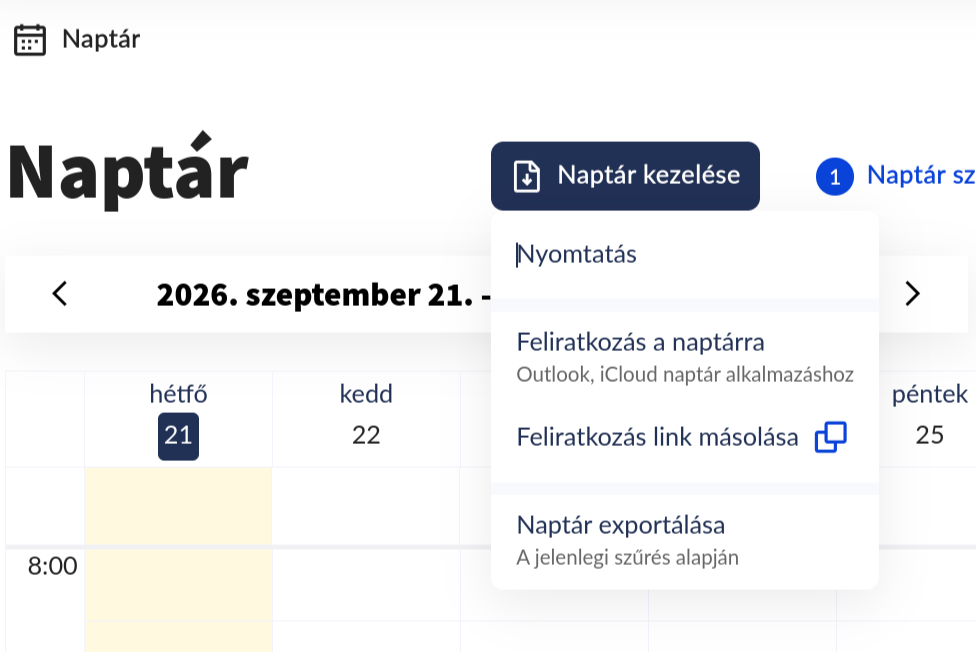
\includegraphics[width=\linewidth]{guide/figures/neptun-calendar-export}
    \caption{Neptun: copy the subscription link.}\label{guide:fig:neptun-export}
  \end{subfigure}\hfill
  \begin{subfigure}[b]{0.3\linewidth}
    \centering
    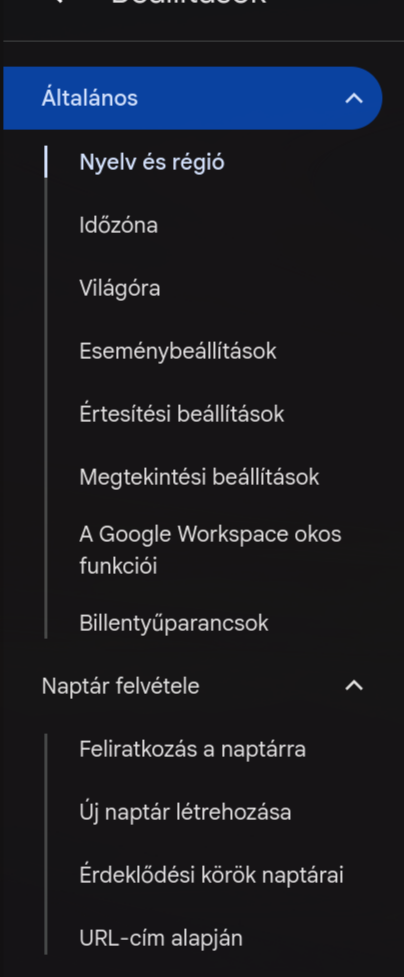
\includegraphics[width=0.75\linewidth]{guide/figures/google-calendar-add-by-url}
    \caption{Google Calendar: add it from the URL.}\label{guide:fig:google-calendar-url}
  \end{subfigure}
  \caption{Subscribe to your Neptun timetable from another calendar.}\label{guide:fig:neptun-calendar}
\end{figure}

\paragraph{Share it with your advisors.} In the Teams calendar, choose \emph{Add calendar} and enter each advisor's name. Ask for permission to view their calendars and share yours with them. We use these to find a weekly slot (\cref{guide:consult}).

\paragraph{Keeping calendars in sync.} We recommend \href{https://reclaim.ai/}{Reclaim.ai} for calendar management. If your university account blocks access, try \href{https://www.outlookgooglecalendarsync.com/}{Outlook Google Calendar Sync}.

%----------------------------------------------------------------------------
\section{Development environment}\label{guide:start:env}
\paragraph{Operating system.} Use Linux or WSL for the command-line tools. macOS uses the Linux-container build route; check the selected tools and container architecture during setup. Native Windows builds are outside the supported route. On WSL, browser and desktop application steps, including the Zotero connector, usually run on the Windows host; the repository and command-line tools run inside WSL.

\paragraph{Editor.} We use \href{https://code.visualstudio.com/}{Visual Studio Code}. Useful extensions include Remote - SSH for the VM, GitHub Pull Requests, Claude Code, Codex and the extensions for your programming languages.

\paragraph{Agent harness.} \Cref{guide:code:ai} recommends the agents and harnesses we use. Start with the lint-first workflow and bounded tasks in \cref{guide:code:agents,guide:code:orchestration}; \cref{guide:code:t3} covers optional T3 setup and practical moves.

\paragraph{Notetaking and task management.} Keep notes in plain Markdown and commit them to GitHub. Obsidian, Tana and Emacs Org mode are options. Track tasks in GitHub issues or Todoist.

\paragraph{Virtual machine and remote work.} In the message with your identifiers, ask us to request a VM in the BME cloud. Verify SSH access alongside early research; start reading and writing while provisioning is in progress. We can provide 8 cores and 16\,GB of memory in the \href{https://cloud.bme.hu/}{BME cloud}, usually in its \href{https://fured.cloud.bme.hu/}{Füred} environment. Host your editor and repositories there, or run AI agents while your laptop is closed. Connect through SSH, RDP, VS Code Remote or Tailscale. Agents and their harnesses (\cref{guide:code:ai}) can run on the VM directly or through remote access. For T3 Connect and the distinction between closing the client and stopping the host, see \cref{guide:code:t3}.

\paragraph{Workspace layout.} Keep one clone of the project repository on your machine or VM. Open the generated \texttt{tdk.code-workspace} in VS Code. The paper, code, proofs, benchmarks, scratch notes and presentation share one commit history. After a consultation, commit its summary in \texttt{scratch/notes/consultations/} together with any agreed source changes. Keep generated outputs and local credentials out of Git.

\paragraph{Do not overdo it.} Limit the time you spend setting up your environment. We learned this the hard way.
